\section{Posteriors of all parameters of the worked example}
\label{app:example}
This appendix shows the posteriors of all parameters of the system of Sec.~\ref{sec:example}, an ET system of the EPL+shear family; Table~\ref{tab:fullpost} lists their true values, medians and 90\% intervals. The Supplemental Material~\cite{supplement} shows the same for an O5 system and lists the true values and posteriors of every analyzed system.

Figure~\ref{fig:cornergw} shows the joint parameter estimation of the two GW images (Sec.~\ref{sec:gwdata}), with the sky position fixed at the host. The two images share the detector-frame chirp mass, the mass ratio, the two aligned spins, the inclination, the polarization angle and the phase. Image $A$ has its own apparent distance $D_A$ and arrival time, and image $B$ is described by the magnification ratio and the delay relative to $A$; the Morse indices of both images are sampled as discrete parameters. All true values lie within the 90\% intervals. The chirp mass is measured to 0.05\% and the delay to 0.2\,ms, i.e. to a fraction $4\times10^{-11}$ of its value of 68 days. The apparent distance has a tail to large values that follows the inclination, the usual distance--inclination degeneracy. The polarization angle and the phase are multimodal, as usual for a signal dominated by the quadrupole mode, which is nearly unchanged by discrete shifts of these angles; the two Morse-index combinations of Sec.~\ref{sec:example}, which differ by a phase shift common to both images, are a related ambiguity. The GW likelihood of the $H_0$ analysis uses only the magnification ratio, the apparent distance, the Morse indices and the delay from this posterior (Sec.~\ref{sec:gwlike}).

Figure~\ref{fig:cornerlens} shows the posterior of the GW+EM analysis with the EPL+shear model: the lens parameters, the external convergence, $h$, and the magnifications that follow from them. The Einstein radius follows the velocity dispersion through the isothermal relation, and at fixed image positions a steeper slope requires a lower velocity dispersion and predicts smaller magnifications and a longer delay per unit $h$, so that $\gamma'$, $\sigma_v$, $\mu_A$, $|\mu_B|$ and $h$ are strongly correlated. The posterior of $\kappa_{\rm ext}$ equals its prior: the data do not constrain the mass sheet (Sec.~\ref{sec:degeneracies}). The lens center and the shear orientation are also determined mainly by their priors; the true center of this lens lies two prior standard deviations from the light center, and its $y$ coordinate is the only parameter outside its 90\% interval. The posterior of $h$ shown here does not include the selection term, which changes the median from 1.13 to 1.12 (Sec.~\ref{sec:example}).

\begin{table}
\caption{True values, medians and 90\% intervals of all parameters of the worked example (Sec.~\ref{sec:example}). Angles are in radians; $t_A$ is the geocentric arrival time of image $A$ and $\Delta t$ the delay of image $B$. For the Morse indices, the posterior probabilities of the two combinations found are given.}
\label{tab:fullpost}
\begin{tabular*}{\linewidth}{@{\extracolsep{\fill}}lccc@{}}
\toprule
Parameter & Truth & Median & 90\% interval\\
\midrule
\multicolumn{4}{@{}l}{\emph{GW: joint parameter estimation, sky position at the host}}\\
Chirp mass $\mathcal M$ ($M_\odot$) & $21.547$ & $21.542$ & $[21.531,\ 21.553]$\\
Mass ratio $m_2/m_1$ & $0.93$ & $0.87$ & $[0.69,\ 0.99]$\\
Spin $\chi_1$ & $-0.36$ & $-0.28$ & $[-0.53,\ -0.12]$\\
Spin $\chi_2$ & $0.03$ & $-0.02$ & $[-0.23,\ 0.23]$\\
Inclination $\theta_{JN}$ & $2.17$ & $2.20$ & $[2.09,\ 2.59]$\\
Polarization $\psi$ & $0.93$ & $1.05$ & $[0.72,\ 2.61]$\\
Phase $\phi_c$ & $1.30$ & $3.68$ & $[0.50,\ 4.57]$\\
$D_A=d_L/\sqrt{|\mu_A|}$ (Gpc) & $8.91$ & $9.34$ & $[8.23,\ 12.76]$\\
$\ln|\mu_B/\mu_A|$ & $-1.23$ & $-1.29$ & $[-1.48,\ -1.10]$\\
$\delta t_A=t_A-t_A^{\rm true}$ (ms) & $0.000$ & $-0.026$ & $[-0.244,\ 0.151]$\\
$\delta\Delta t=\Delta t-\Delta t^{\rm true}$ (ms) & $0.000$ & $0.071$ & $[-0.128,\ 0.289]$\\
Morse indices $(n_A,n_B)$ & $(0,\frac12)$ & \multicolumn{2}{c}{$(0,\tfrac12)$: 0.53; $(\tfrac12,1)$: 0.47}\\
\midrule
\multicolumn{4}{@{}l}{\emph{GW+EM: EPL+shear lens model, $\kappa_{\rm ext}$ and $h$}}\\
$\theta_E$ (arcsec) & $0.642$ & $0.605$ & $[0.563,\ 0.647]$\\
Radial slope $\gamma'$ & $1.93$ & $2.05$ & $[1.88,\ 2.27]$\\
Axis ratio $q$ & $0.85$ & $0.87$ & $[0.79,\ 0.94]$\\
Orientation $\varphi$ & $2.13$ & $2.11$ & $[1.86,\ 2.37]$\\
Shear $\gamma_{\rm ext}$ & $0.047$ & $0.038$ & $[0.016,\ 0.076]$\\
Shear orientation $\varphi_{\rm ext}$ & $0.80$ & $0.75$ & $[0.11,\ 2.97]$\\
Center $x_c$ (arcsec) & $0.002$ & $0.001$ & $[-0.030,\ 0.032]$\\
Center $y_c$ (arcsec) & $0.041$ & $-0.006$ & $[-0.035,\ 0.023]$\\
$\sigma_v$ (km\,s$^{-1}$) & $221$ & $215$ & $[207,\ 222]$\\
$\kappa_{\rm ext}$ & $0.000$ & $-0.001$ & $[-0.042,\ 0.041]$\\
$\mu_A$ & $3.21$ & $2.43$ & $[1.72,\ 3.89]$\\
$|\mu_B|$ & $0.94$ & $0.68$ & $[0.44,\ 1.12]$\\
$h=H_0/H_0^{\rm true}$ & $1.00$ & $1.13$ & $[0.94,\ 1.29]$\\
\bottomrule
\end{tabular*}

\end{table}

\begin{figure*}
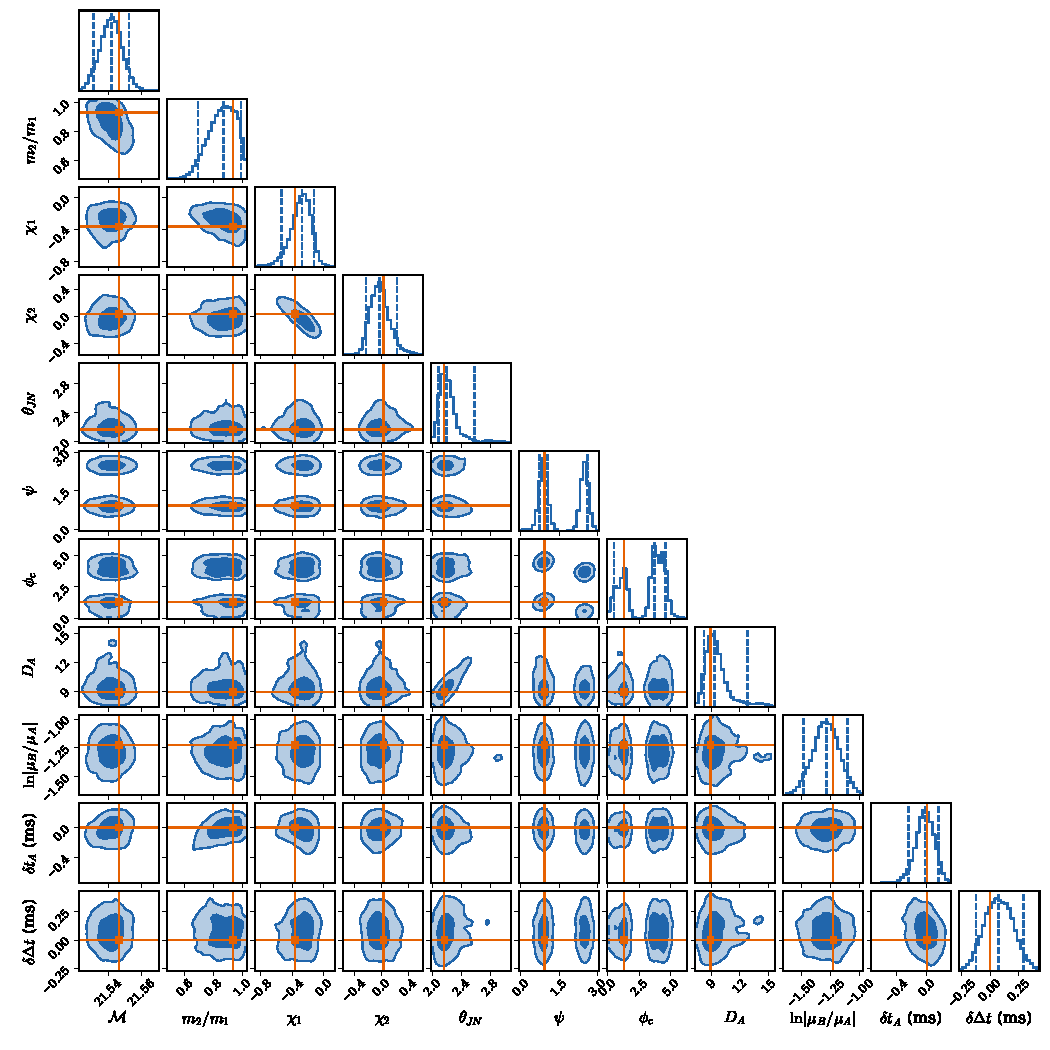
\includegraphics[width=\textwidth]{fig_corner_gw.pdf}
\caption{Joint parameter estimation of the two GW images of the worked example, with the sky position fixed at the host: detector-frame chirp mass $\mathcal M$ (in $M_\odot$), mass ratio, aligned spins, inclination, polarization angle and phase (in rad), apparent distance of image $A$ (in Gpc), magnification ratio, and the offsets of the arrival time of $A$ and of the delay from their true values (in ms). Contours enclose 50\% and 90\% of the posterior; dashed lines mark the medians and 90\% intervals, and orange lines the true values.}
\label{fig:cornergw}
\end{figure*}

\begin{figure*}
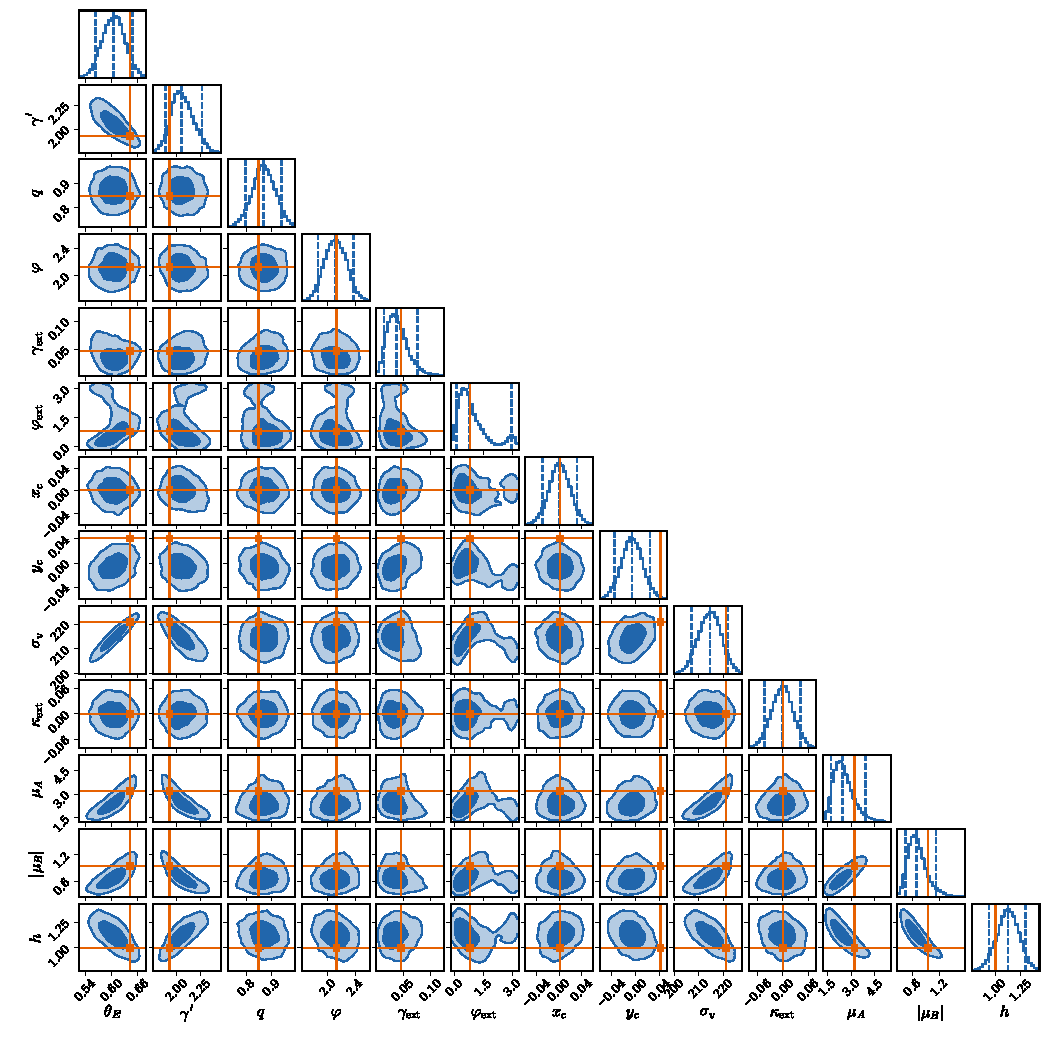
\includegraphics[width=\textwidth]{fig_corner_lens.pdf}
\caption{GW+EM posterior of the worked example with the EPL+shear model: Einstein radius and lens center (in arcsec), slope, axis ratio and orientation of the mass, shear strength and orientation, velocity dispersion (in km\,s$^{-1}$), external convergence, the magnifications of the two images, and $h$ (without the selection term). Lines and contours as in Fig.~\ref{fig:cornergw}.}
\label{fig:cornerlens}
\end{figure*}

\section{Calibration of the per-system posteriors}
\label{app:calibration}
If the per-system posteriors of $h$ are calibrated, the posterior probability below the true value, $P(h<1|d_i)$, is uniformly distributed over the systems, and a fraction 0.9 of the 90\% intervals contain the truth. Figure~\ref{fig:pit} shows both diagnostics for the analyses with the model of the simulated family and the selection term. The distribution of $P(h<1|d_i)$ is consistent with uniform for both scenarios: its mean is 0.43 (ET) and 0.51 (O5), and the Kolmogorov--Smirnov distances from the uniform distribution, 0.13 and 0.09, are below the 5\% critical value of 0.18 for 60 systems. The coverage of the 90\% intervals depends on the magnification of the brighter GW image. Below $|\mu|\approx5$ it is consistent with 0.9 in every bin; above, it drops to about 0.7 for the O5 systems, of which 37 of 59 lie in this range (ET has only 6). For these near-caustic systems the delay and the magnifications depend steeply on the source position and the lens parameters. A plausible cause, which we have not tested, is the linearized image-position likelihood of the lens reconstruction (Paper~I, Appendix~C), which assumes that the lensing Jacobian is constant over the astrometric uncertainty of each image; near a fold this assumption fails. The combined estimate of Sec.~\ref{sec:joint} is not biased at the present precision, because the shortfall is in the widths and not systematically in the medians, but a sample of several hundred O5 systems would require a calibrated likelihood for these systems.

\begin{figure}
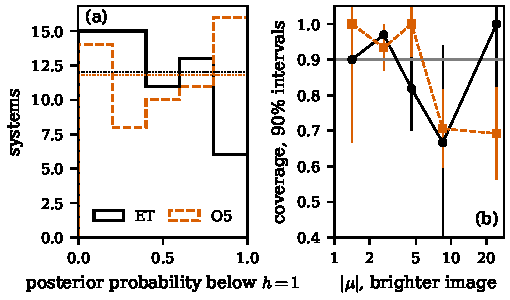
\includegraphics[width=\columnwidth]{fig_pit.pdf}
\caption{Calibration of the per-system posteriors of $h$ (model of the simulated family, with the selection term). (a) Distribution over systems of the posterior probability below the true value, for ET (solid) and O5 (dashed); the dotted lines mark the uniform expectation. (b) Fraction of the 90\% intervals that contain the truth, in bins of the magnification of the brighter GW image, with binomial errors; the line marks 0.9.}
\label{fig:pit}
\end{figure}

\section{Strain-level check of the two-stage likelihood}
\label{app:full}
The analyses of this paper use the joint parameter-estimation posterior of each system as an effective likelihood: a Gaussian in $(\ln\mu_B/\mu_A,\ln D_A)$ times the probabilities of the Morse indices (Sec.~\ref{sec:gwlike}). To test this approximation, we also sampled the strain likelihood of both images together with the lens model, so that the lens parameters determine the magnifications, Morse indices and delay of the injected waveforms directly. These full analyses use the same noise realizations, priors and lens likelihood, with 300 live points, and a free sky position for both scenarios. We compare the posteriors of the magnification of image $A$, $\ln\mu_A$, by the difference of the medians in units of the standard deviation of the full posterior, estimated from its 90\% interval, and by the ratio of the interval widths. Systems whose GW data in the full analysis differ from those of the parameter estimation (a different noise realization, or for one O5 system the two images injected with the other labels) are excluded.

Without a cosmology, where the GW data enter only through the magnification ratio, the Morse indices and the arrival order (the setting of Paper~I), the medians of 40 ET and 39 O5 systems differ by a median of 0.15 and 0.05 standard deviations, by more than one standard deviation for 7.5\% of the ET systems and none of the O5 systems, and the widths agree to 2\% and 3\%. In flat $\Lambda$CDM at the true $H_0$, where the apparent distance also enters, we compared 55 systems analyzed with the EPL+shear model and $\sigma_{\kappa_{\rm ext}}=0.025$. For the 25 O5 systems the medians differ by a median of 0.16 standard deviations, by more than one standard deviation for none, and the widths by 8\%. For the 30 ET systems the median difference is 0.34 standard deviations, and 20\% differ by more than one. With a free sky position the ET posteriors favor several sky positions (Paper~I), with correspondingly different antenna responses and apparent distances, which a single Gaussian probably represents poorly. The ET analyses of this paper use the host sky position, for which the parameter-estimation posteriors of the magnification ratio and apparent distance pass the calibration tests of Paper~I. Moreover, Sec.~\ref{sec:information} shows that removing the apparent distance from the likelihood altogether changes the per-system $h$ by a median of only 0.16 standard deviations, so the results for $H_0$ are insensitive to the accuracy of the distance summary.
